\documentclass[doc, a4paper, apacite]{apa6}

\usepackage[american]{babel}

\usepackage{csquotes}
%\usepackage[style=apa,sortcites=true,sorting=nyt,backend=biber]{biblatex}
%\DeclareLanguageMapping{american}{american-apa}
\usepackage{threeparttable}
\usepackage{booktabs} % For nice tables
\usepackage{amsmath} % For \text{} function 
\usepackage{setspace}

\title{Decision-making and communication under uncertainty}
\shorttitle{DSTL07: Sensitivity to uncertainty}

\author{Charlotte E. R. Edmunds, Andy J. Wills, Adam Harris, Magda Osman}
\affiliation{Queen Mary, UCL, University of London \\ 11 January 2021}

%\leftheader{Edmunds}

%\abstract{}
%
%\keywords{}

\begin{document}
\maketitle
	\doublespacing
	
\section{Method}

\subsection{Participants}
Participants were recruited through Prolific Academic.
We limited the sample to participants between the ages of 18 and 65 with corrected to normal vision. 
Participants were paid a flat fee of \pounds 2 for completing the learning phase.
Those that passed the learning phase were given a bonus of \pounds 6 if they then completed the following two test phases. 

This sample size was based on an \emph{a priori} statistical power analysis using G*Power 3.1 \cite{GPower2007, GPower2009}. 
We assumed a medium effect size (partial $\eta^2 = .06$) with $\alpha=0.05$ and power $(1-\beta)= 0.95$.
The projected total sample size was $N=206$.
We rounded this up to $N=208$ so to have even numbers of participants in each experimental group. 

\subsection{Category structure}
The abstract category structure that all participants learned is shown in Table~\ref{table:abstractStructure}. 
The stimuli are constructed from five binary dimensions. 
In the experiment, Category X and Y will be randomly assigned to the labels `Friendly' and `Hostile.' 
In addition, the dimensions will be randomly assigned to the label (and therefore perceptual features) of Craft (airplane, submarine), Speed (fast, slow), Direction (left, right), Type (autonomous, decoy) and Status (fully operational, damaged). 

\begin{table}[t]
	\centering
	\caption{}
	\label{table:abstractStructure}
	\begin{tabular}{lllllllllll}
		\toprule
		\multicolumn{5}{c}{Category X} &  & \multicolumn{5}{c}{Category Y} \\
		\cline{1-5} \cline{7-11} \\
		D1   & D2   & D3   & D4  & D5  &  & D1   & D2   & D3   & D4  & D5  \\
		\midrule
		1    & 1    & 1    & 1   & 1   &  & 0    & 0    & 0    & 0   & 0   \\
		1    & 1    & 1    & 1   & 0   &  & 0    & 0    & 0    & 0   & 1   \\
		1    & 1    & 1    & 0   & 1   &  & 0    & 0    & 0    & 1   & 0   \\
		1    & 1    & 1    & 0   & 0   &  & 0    & 0    & 0    & 1   & 1   \\
		1    & 1    & 0    & 1   & 1   &  & 0    & 0    & 1    & 0   & 0   \\
		1    & 1    & 0    & 1   & 0   &  & 0    & 0    & 1    & 0   & 1   \\
		1    & 1    & 0    & 0   & 1   &  & 0    & 0    & 1    & 1   & 0   \\
		1    & 0    & 1    & 1   & 0   &  & 0    & 1    & 0    & 0   & 1   \\
		1    & 0    & 1    & 0   & 1   &  & 0    & 1    & 0    & 1   & 0   \\
		0    & 1    & 1    & 1   & 0   &  & 1    & 0    & 0    & 0   & 1   \\
		\bottomrule
	\end{tabular}	
\end{table}

\begin{figure}[b]
	\centering
	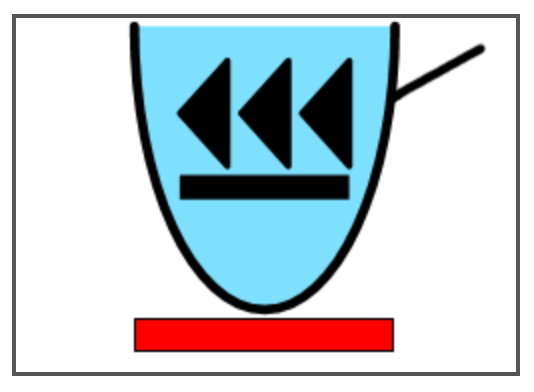
\includegraphics[width=0.33\textwidth]{images/integratedStimulusExample}
	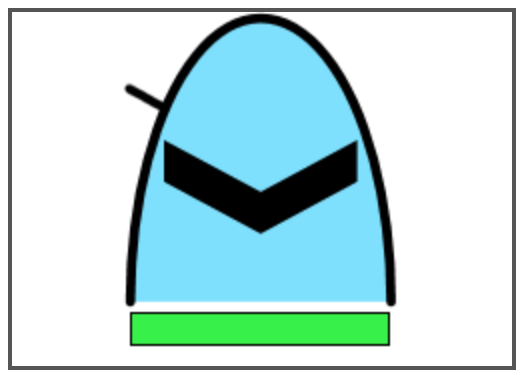
\includegraphics[width=0.33\textwidth]{images/integratedStimulusExample2}
	\caption{Example of stimulus dimensions as integrated stimuli.}
	\label{fig:integratedStimuli}
\end{figure}

\subsection{Design}
The experiment had a 2 (spatial presentation: separated, integrated) x 2 (social: operator, superior) between-subjects design. 

Participants were randomly assigned to see the stimuli as either spatially integrated (as in Figure~\ref{fig:integratedStimuli}) or spatially separated (as in Figure~\ref{fig:separatedStimulus}). 
Additionally, they were either told that their confidence ratings are to be given to their commander or to one of their fellow operators. 

\begin{figure}[t]
	\centering	
	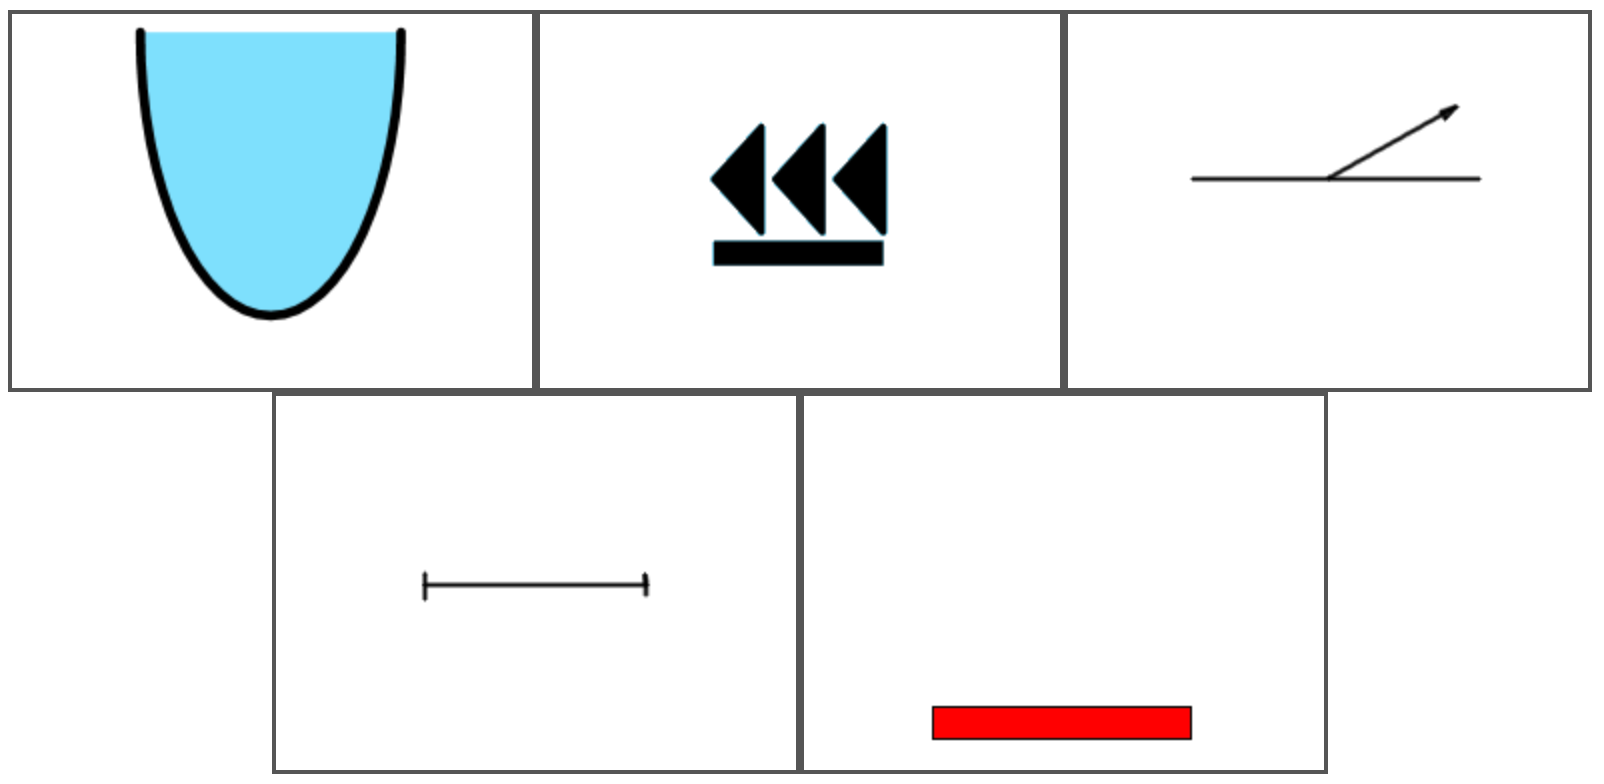
\includegraphics[width=0.6\textwidth]{images/separatedStimulusExample}
	\caption{An example stimulus presented as a separated set of symbols.}
	\label{fig:separatedStimulus}	
\end{figure}

\subsection{Procedure}
At the beginning of the experiment, participants were welcomed and told where to write to if they had any queries or concerns. 
The experiment had three blocks of trials: a learning phase and two types of test phase. 

\subsubsection{1. Category learning} 
Participants were told the overall structure of the experiment and told what each of the perceptual features of the glyph represent. 
They were then given specific instructions for the category learning phase. 
On each trial they were shown a stimulus (either separated or integrated depending on the condition they were assigned).
They then had to click one of two buttons labelled `Friendly' or `Hostile' to make their response.
Then they were shown the feedback `Correct!' or `Wrong', as appropriate, for $1000ms$.
This was followed by a blank screen for $500ms$.

The stimuli in this section were pseudo-randomised so every 20 trials the participants saw all the training stimuli in a random order. 
Participants were trained to a learning criterion of 80\% correct in the last 20 trials. 
Thus, the fewest number of trials a participant could see were 20 trials. 
Participants who did not exceed the learning criterion in 200 trials were excluded from the rest of the experiment. 

\subsubsection{2. Test with all dimensions}
After a short, self-paced break, participants moved to the second phase. 
Here, participants were tested on all 32 stimuli created from the binary levels of 5 stimulus dimensions. 
In this phase, there were 5 rounds, where participants saw all 32 stimuli in a random order. 
On every trial, they saw a stimulus and had to click on one of two buttons to indicate whether they thought it was friendly or hostile. 
No feedback was provided. 
On every 4 trials, starting from the first trial, participants were also asked to rate their confidence in the category judgment they had just given. 
Participants rated their confidence using a slider that went from `No idea' to `Certain.'
The data from this scale was discretised into 100 levels. 
There was an inter-trial interval of 500ms. 

Following this, there was an opportunity for participants to inform us how they completed the task. 
We reminded them of what the levels of each stimulus dimension meant, then we asked them to rank the five stimulus dimensions based on how important they were for classification. 
Then, we provided an open text box and asked participants to describe how exactly they decided whether a craft was friendly or hostile in the previous task.

\subsubsection{3. Test removing a dimension}
The final test phase was identical to the previous one in all but one respect: the stimuli shown to the participant only had four dimensions. 
In this final test phase, we removed the dimension that was 90\% predictive for that participant. 
For participants in the integrated condition, it was simply absent from the display. 
For participants in the separated condition, the box was filled with the text ``Information not available.''

\section{Results}

\subsection{Learning phase}
\subsubsection{Trials to criterion}
Here, we analyse the number of trials it took for participants to reach the learning criterion as shown in Figure~\ref{fig:DSTL07trialsCriterion}. 
For each condition, we removed outlying participants, i.e. those who took more trials than the upper quartile plus 1.5 times the interquartile range. 
This resulted in removing 3 participants from the integrated-operator condition, 2 from the integrated-superior condition and 7 from the separated-operator condition. 

Levene's test showed homogeneity of variance was violated, $F(3,195)=7.98$, $p<.001$.
Similarly, a Shapiro-Wilks test showed the data violated assumptions of normality, $W=0.89$, $p<.001$. 
Therefore, to correct for the violation of the normality assumption, we report an ANOVA based on the log transformed number of trials to criterion and its Bayesian equivalent. 
The ANOVA found a hint of an interaction between display condition and social condition, $BF=1.39905$, $F(1, 195)=4.33$, $p=.039$. 
There was a greater difference between the display conditions in the superior conditions, $M_\text{integrated}=3.64$, $SE=0.09$, $M_\text{separated}=3.89$, $SE=0.08$, than in the operator conditions, $M_\text{integrated}=3.51$, $SE=0.09$, $M_\text{separated}=3.40$, $SE=0.09$. 
The interaction was moderated by a main effect of social condition, $BF=53.66$, $F(1, 195)=12.74$, $p<.001$. 
Participants took longer to learn in the operator condition, $M=3.45$, $SE=0.06$, than in the superior condition, $M=3.76$, $SE=0.06$. 
The effect of display condition did not reach significance, $BF=0.24$, $F(1, 195)=1.054$, $p=.306$. 

\begin{figure}
	\centering
	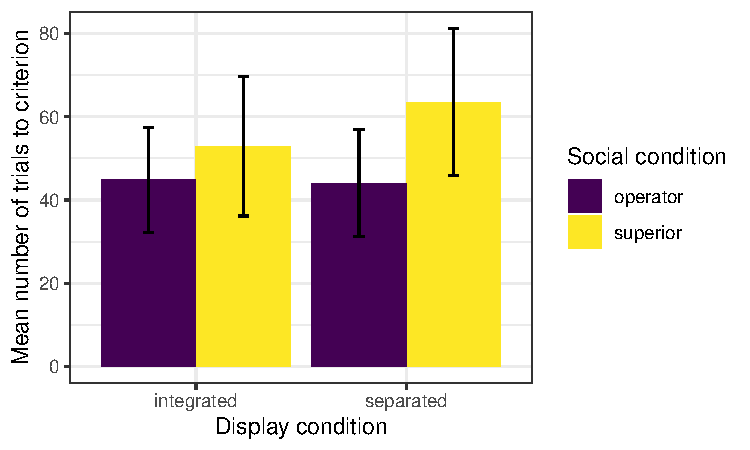
\includegraphics{images/DSTL07trialsCriterion}
	\caption{Mean number of trials to reach the criterion for participants in each condition. Error bars are difference-adjusted confidence intervals.}
	\label{fig:DSTL07trialsCriterion}
\end{figure}


\subsubsection{Reaction times}
Here, we analyse the reaction time during the learning phase of the experiment as shown in Figure~\ref{fig:DSTL07learningRT}. 
For each participant, we removed outlying trials, i.e. those who took more time than the upper quartile plus 1.5 times the interquartile range. 



\begin{figure}
	\centering
	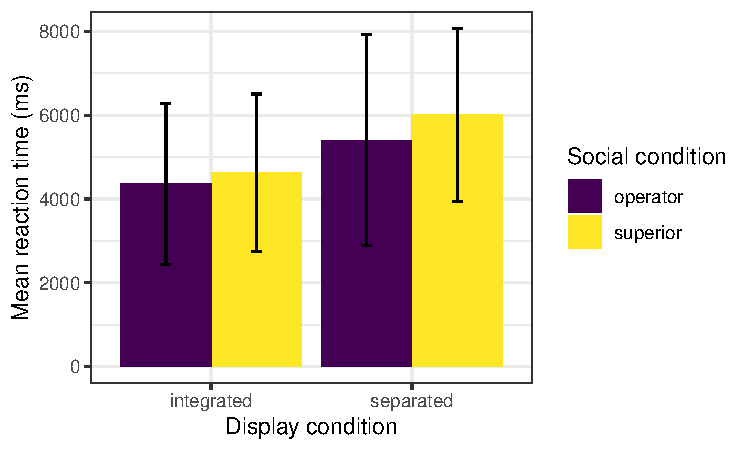
\includegraphics{images/DSTL07learningRT}
	\caption{Mean reaction time in milliseconds for participants in each condition. Error bars are difference-adjusted confidence intervals.}
	\label{fig:DSTL07learningRT}
\end{figure}

\clearpage
\newpage
\bibliographystyle{apacite}
\bibliography{references}

\end{document}
